%!TEX TS-program = xelatex
\documentclass[]{friggeri-cv}
\usepackage{afterpage}
\usepackage{hyperref}
\usepackage{graphicx}
\usepackage{color}
\usepackage{xcolor}
\usepackage{fancyhdr}
\pagestyle{fancy}
\fancyfoot{}
\renewcommand{\headrulewidth}{0pt}
\renewcommand{\footrulewidth}{0.4pt}
\fancyfoot[LE,RO]{\thepage}
\fancyfoot[RE,LO]{Jyotirmoy Das, Ph.D.}
\usepackage[document]{ragged2e}
\hypersetup{
    pdftitle={CV},
    pdfauthor={Jyotirmoy Das},
    pdfsubject={},
    pdfkeywords={},
    colorlinks=false,       % no lik border color
   allbordercolors=white    % white border color for all
}
\addbibresource{bibliography.bib}
\RequirePackage{xcolor}
\definecolor{pblue}{HTML}{0395DE}

\ifxetex
\usepackage{letltxmacro}
\setlength{\XeTeXLinkMargin}{1pt}
\LetLtxMacro\SavedIncludeGraphics\includegraphics
\def\includegraphics#1#{% #1 catches optional stuff (star/opt. arg.)
	\IncludeGraphicsAux{#1}%
}%
\newcommand*{\IncludeGraphicsAux}[2]{%
	\XeTeXLinkBox{%
		\SavedIncludeGraphics#1{#2}%
	}%
}%
\fi

\begin{document}
\header{Jyotirmoy} {Das}
      {Ph.D. (Tech.) in Bioinformatics}
      
% Fake text to add separator      
\fcolorbox{white}{gray}{\parbox{\dimexpr\textwidth-2\fboxsep-2\fboxrule}{%
.....
}}

% In the aside, each new line forces a line break
\begin{aside}
~
~
~
~
~
  \section{Address}
    Befälsgatan 12
    587 50, Linköping, Sweden
    ~
  \section{Tel \& Skype}
    +46 (0)76-136 96 45
    
\includegraphics[scale=0.01]{img/skype}{\textbf{jyotirmoy82}}
    ~
  \section{Mail}
    \href{mailto:jyotirmoy.das@liu.se}{\textbf{jyotirmoy.das@}\\liu.se}
    \href{mailto:jyotirmoy21@gmail.com}{\textbf{jyotirmoy21@}\\gmail.com}
    ~
  \section{Web \& Git}
    \href{https://jyotirmoydas.ucraft.net}{jyotirmoy21.ucraft.net}
    \href{https://github.com/JD2112}{github.com/JD2112}
    ~
  \section{Programming}
    \textbf{R}
\includegraphics[scale=0.40]{img/5stars.png}
   \textbf{Perl}
\includegraphics[scale=0.40]{img/3stars.png}
   \textbf{Python}
\includegraphics[scale=0.40]{img/2stars.png}
   \textbf{Shell}
\includegraphics[scale=0.40]{img/5stars.png}
   \textbf{C/C++}
\includegraphics[scale=0.40]{img/2stars.png}    
   \textbf{HTML}
\includegraphics[scale=0.40]{img/5stars.png}
   \textbf{Markdown}
\includegraphics[scale=0.40]{img/5stars.png} 
    \textbf{Others}
\includegraphics[scale=0.40]{img/5stars.png}
    ~
  \section{OS Handling}
    \textbf{GNU/Linux}
\includegraphics[scale=0.40]{img/5stars.png}
    \textbf{Unix}
\includegraphics[scale=0.40]{img/5stars.png}
    \textbf{MacOS}
\includegraphics[scale=0.40]{img/5stars.png}
    \textbf{HPC}
\includegraphics[scale=0.40]{img/5stars.png}
    \textbf{Windows}
\includegraphics[scale=0.40]{img/5stars.png} 
~
 \section{Skills}
	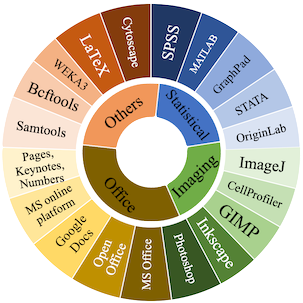
\includegraphics[scale=0.75]{img/skill.png}       
\end{aside}

\section{Experiences}
\begin{entrylist}
\entry
    {2020 - now}
    {Principal Research Engineer}
    {Linköping University, Sweden}
    {Networking and developing computational pipelines to analyze different sequencing techniques.}
  \entry
    {2017 - 2020}
    {Postdoctoral Researcher}
    {Linköping University, Sweden}
    {Designing and developing computational pipelines to study human methylome, transcriptome obtained analyzed using different Illumina platforms in linuxOS.}
  \entry
    {2014 - 2017}
    {Senior Research Fellow}
    {DST-INSPIRE (Govt. of India), Bose Institute, India}
    {Part of PhD program.}
    \entry
    {2012 - 2014}
    {Junior Research Fellow}
    {DST-INSPIRE (Govt. of India), Bose Institute, India}
    {Part of PhD program.}
    \entry
    {2010 - 2012}
    {Institute Fellow}
    {DST-INSPIRE (Govt. of India), Bose Institute, India}
    {Learn programming in MATLAB\textsuperscript{\textregistered}  and work with protein structure and dynamics. Use R to study the co-expression gene network.}
    \entry
    {2009 - 2010}
    {Research Trainee}
    {National Institute of Plant Genome Research, New Delhi, India}
    {Develop new DNA markers (Intron Length Polymorphism) using \textit{Setaria italica} genome.}
\end{entrylist}

\section{Education}
\begin{entrylist}
  \entry
    {2012 - 2017}
    {PhD (Tech) Degree in Bioinformatics}
    {Maulana Abul Kalam Azad University of Technology, West Bengal (Formerly known as West Bengal University of Technology), India}
    {Molecular Evolution and MicroRNAs.\\
    Main subjects: Comutational Biology, Human Diseases.\\
    \emph{Title of the Thesis: "In-silico studies of MicroRNA Regulations in higher eukaryotes from the perspective of Molecular Evolution" \href{http://library.wbut.ac.in/cgi-bin/koha/opac-retrieve-file.pl?id=579ff58a1245f1e3890d618e10f5cbad}{(PDF Link)}   .}\\
    \emph{Supervisor: Prof. Tapash C Ghosh, Bose Institute, India.}\\}
  \entry
    {2008 - 2010}
    {Master of Technology in Biotechnology}
    {West Bengal University of Technology, India}
    {Main subject: Biotechnology.\\
    \emph{Title of the Thesis: "Identification and evaluation of Intron Length Polymorphism (ILP) marker in Foxtail millet (Setaria italica) and to study evolutionary relationship between species by cross-species transferability".}\\
    \emph{Supervisors: Dr. Manoj Prasad, NIPGR, India. Prof. Nandan Bhattacharyya, Haldia Institute of Technology, India}\\}
 \entry
	{2006 - 2008}
	{Master of Science in Biotechnology}
	{Bangalore University, Karnataka, India}
	{Main subject: Biotechnology.\\}
\entry
	{2003 - 2006}
	{Bachelor of Science in Biotechnology}
	{University of Kalyani, West Bengal, India}
	{Main subjects: Biotechnology, Chemistry and Computer Applications.\\
	\emph{Project 1: "Drug Designing: Evaluation of iron chelation through blood in phytic acid treated thalassemia patients".}\\
	\emph{Project 2: "Study of Ecological Diversity in Sunderbans, Especially on Kingfishers"}\\
	\emph{Supervisors: Prof. Amit Chakravorty, Dr. Sudipa Chakravorty, IGE, India}\\}
\end{entrylist}
\newpage
\section{Certifications}
\begin{entrylist}

  \entry
    {2020}
    {Research Supervision}
    {Linköping University Pedagogy Course}
	
\entry
	{2019}
	{Becoming a Teacher in Higher Education }
	{Linköping University Pedagogy Course}	
    
 \entry
	{2015}
	{Astrobiology and the Search for Extraterrestrial Life}
	{Coursera e-learning}
	{\emph{The origin and evolution of life and the search for life beyond the Earth. \href{https://coursera.org/share/69979189b92c63a21c48390547f60df1}{(Link to Certificate)}}}
	
\entry
	{2015}
	{Programming for Everybody (Getting Started with Python)}
	{Coursera e-learning}
	{\emph{Building a Python fundamental. \href{https://coursera.org/share/69979189b92c63a21c48390547f60df1}{(Link to Certificate)}}}
	

\end{entrylist}

\section{Publications}
\begin{entrylist}
\entry
	{2021}
	{\underline{Das J}, Paues J, Idh N, Pehrson I, Lerm M}
	{submitted}
	{\textbf{A DNA methylome biosignature in alveolar macrophages from TB-exposed individuals predicts exposure to mycobacteria}\\
	\emph{medRxiv}\\ \href{https://www.medrxiv.org/content/10.1101/2021.03.16.21253732v1.full.pdf}{doi.org/10.1101/2021.03.16.21253732}}
\entry
	{2021}
	{Pehrson I, \underline{Das J}, Idh N, Karlsson L, Rylander H, Segerstad HH, Reuterswärd E, Marttala E, Paues J, Méndez-Aranda M, Ugarte-Gil C, Lerm M}
	{submitted}
	{\textbf{DNA methylomes derived from alveolar macrophages display distinct patterns in latent tuberculosis-implication for interferon gamma release assay status determination}\\
	\emph{medRxiv}\\ \href{https://www.medrxiv.org/content/10.1101/2021.03.16.21253725v1.full.pdf}{doi.org/10.1101/2021.03.16.21253725}}
\entry
	{2021}
	{Huoman J, Sayyab S, Apostolou E, Karlsson L, Porcile L, Rizwan M, Sharma S, \underline{Das J}, Rosen A, Lerm M}
	{submitted}
	{\textbf{Mild SARS-CoV-2 infection modifies DNA methylation of peripheral blood mononuclear cells from COVID-19 convalescents}\\
	\emph{medRxiv}\\ \href{https://www.medrxiv.org/content/10.1101/2021.07.05.21260014v1.full.pdf}{doi.org/10.1101/2021.07.05.21260014}}
\entry
	{2021}
	{Pehrson I, Braian C, Karlsson L, Idh N, Danielsson EK, Andersson B, Paues J, \underline{Das J}, Lerm M}
	{submitted}
	{\textbf{DNA methylation profiling of immune cells from tuberculosis-exposed individuals overlaps with BCG-induced epigenetic changes and correlates with the emergence of anti-mycobacterial ‘corralling cells’}\\
	\emph{medRxiv}\\ \href{https://www.medrxiv.org/content/10.1101/2021.09.01.21262945v1.full.pdf}{doi.org/10.1101/2021.09.01.21262945}}
\entry
	{2021}
	{Singhania A, Dubelko P, Kuan R, Chronister WD, Muskat K, \underline{Das J}, Phillips EJ, Mallal SA, Seumois G, Vijayanand P, Sette A, Lerm A, Peters B, Arlehamn CSL}
	{accepted in eBioMedicine}
	{\textbf{CD4+ CCR6+ T cells dominate the BCG-induced transcriptional signature}\\
	\emph{medRxiv}\\ \href{https://www.biorxiv.org/content/10.1101/2021.08.20.457054v1.full.pdf}{doi.org/10.1101/2021.08.20.4570545}}
\end{entrylist}

\begin{aside}
~
~
~
~
  \section{Invited reviewer}
	IJERPH [1]
	International Journal of Molecular Sciences [2]
	Genomics [1]
	Genes \& Genomics [1]
	Cancer Mangement and Research [2]
	Journal of Biomolecular Structure \& Dynamics [1]
	Peer J [1]
 ~
  \section{Supervision}
  \textbf{Main Supervisor:} Master students [2]
  ~
  \textbf{Co-supervisor:} Master students [9], PhD students [2]
 ~ 
\section{Collaborations}
\textbf{Internal}
	Dr. Mika Gustafsson, Bioinformatics, LiU [One Article]
	~
	Dr. Deepti Verma, Cell Biology, LiU [One Manuscript]
	~
	Prof. Peter Söderkvist, Cell Biology, LiU [One manuscript]
~
  \section{Instruments}
  Pyrosequencer MD96
  ThermalCycler
  IncuCyte\textsuperscript{\textregistered}
~  
\end{aside}

\newpage
\section{Publications...conitnue}
\begin{entrylist}
\entry
	{2021}
	{\underline{Das J}, Idh N, Sikkeland LIB, Paues J, Lerm M}
	{IF: 5.171; Citations: 4}
	{\textbf{DNA methylome-based validation of induced sputum as an effective protocol to study lung immunity: construction of a classifier of pulmonary cell types}\\
	\emph{Epigenetics, Sep 5:1-12}\\ \href{https://www.tandfonline.com/doi/pdf/10.1080/15592294.2021.1969499}{doi: 10.1080/15592294.2021.1969499}}
\entry
	{2021}
	{Karlsson L, \underline{Das J}, Nilsson M, Tyrén A, Pehrson I, Idh N, Sayyab S, Paues J, Ugarte-Gil C, Méndez-Aranda M, Lerm M}
	{IF: 5.133; Citations: 1}
	{\textbf{A differential DNA methylome signature of pulmonary immune cells from individuals converting to latent tuberculosis infection}\\
	\emph{Sci Rep 11, 19418}\\ \href{https://www.nature.com/articles/s41598-021-98542-3.pdf}{doi.org/10.1038/s41598-021-98542-3}}
\entry
	{2021}
	{Kalsum K, Andersson B, \underline{Das J}, Schön T, Lerm M}
	{IF: 3.605; Citations: 1}
	{\textbf{A differential DNA methylome signature of pulmonary immune cells from individuals converting to latent tuberculosis infection}\\
	\emph{BMC Microbiol 21, 167}\\ \href{https://www.nature.com/articles/s41598-021-98542-3.pdf}{doi.org/10.1038/s41598-021-98542-3}}
\entry
	{2021}
	{Zhu GH, Azharuddin M, Islam R, Rahmoune H, Deb S, Kanji U, \underline{Das J}, Osterrieth J, Aulakh P, Ibrahim-Hashi H, Manchanda R, Nilsson PH, Mollnes TE, Bhattacharyya M, Islam MM, Hinkula J, Slater NKH, Patra HK}
	{IF:  9.229; Citations: 0}
	{\textbf{Innate Immune Invisible Ultrasmall Gold Nanoparticles—Framework for Synthesis and Evaluation}\\
	\emph{ACS Appl. Mater. Interfaces 13, 20, 23410–23422}\\ \href{https://pubs.acs.org/doi/pdf/10.1021/acsami.1c02834}{doi.org/10.1021/acsami.1c02834}}
\entry	
	{2019}
	{\underline{Das J}, Verma D, Gustafsson M, Lerm M}
	{IF: 5.171; Citations: 13}
	{\textbf{Identification of DNA methylation patterns predisposing for an efficient response to BCG vaccination in healthy BCG-naïve subjects}\\
	\emph{Epigenetics, Vol 14, Issue 6, 589 - 601}\\ \href{https://www.tandfonline.com/doi/pdf/10.1080/15592294.2019.1603963?needAccess=true}{https://doi.org/10.1080/15592294.2019.1603963}}
\entry
	{2018}
	{Sen K, Bhattacharyya D, Sarkar A, \underline{Das J}, Maji N, Basu M, Ghosh Z, Ghosh TC}
	{IF: 3.681 ; Citations: 6}
	{\textbf{Exploring the major cross-talking edges of competitive endogenous RNA networks in human Chronic and Acute Myeloid Leukemia}\\
	\emph{Biochim Biophys Acta, Gen Subj, 1862 (9): 1883 – 1892}\\ \href{https://doi.org/10.1016/j.bbagen.2018.06.002}{https://doi.org/10.1080/15592294.2019.1603963}}
\entry
	{2014}
	{\underline{Das J}, Podder S, Ghosh TC}
	{IF: 3.986; Citations: 37}
	{\textbf{Insights into the miRNA regulations in human disease genes.}\\
	\emph{BMC Genomics, 15:1010.}\\ \href{https://bmcgenomics.biomedcentral.com/track/pdf/10.1186/1471-2164-15-1010}{https://doi.org/10.1186/ 1471-2164-15-1010}}
\entry
	{2013}
	{\underline{Das J}, Chakraborty S, Podder S, Ghosh TC}
	{IF: 3.805; Citations: 7}
	{\textbf{Complex-forming proteins escape the robust regulations of miRNA in Human.}\\
	\emph{FEBS Lett 587(14):2284-7.}\\ \href{https://www.sciencedirect.com/science/article/pii/S0014579313004419}{https://doi.org/10.1016/j.febslet.2013.05.062}}
\entry
	{2011}
	{Gupta S, Kumari K, \underline{Das J}, ..., Prasad M}
	{IF: 2.152; Citations: 49}
	{\textbf{Development and utilization of novel intron length polymorphic markers in foxtail millet (Setaria italica (L.) P. Beauv.).}\\
	\emph{Genome 54(7): 586-602.}\\
	 \href{https://doi.org/10.1139/g11-020}{https://doi.org/10.1139/g11-020\\}}
\end{entrylist}


\begin{aside}
~
~
~
~
  \section{Networks}
	SciLifeLab, Sweden
	Clinical Genomics, Sweden
	Genomic Medicine, Sweden
 ~
  \section{Container handling}
	Conda
	Singularity
	Docker
	Podman	
~ 
~ 
\section{Community}
\textbf{github}
~
	\href{https://github.com/Lerm-Lab}{Lerm-Lab}
	~
	\href{https://github.com/Genomic-Medicine-Linkoping}{Genomic-Medicine-Linkoping}
	~
	\href{https://github.com/genomic-medicine-sweden}{genomic-medicine-sweden}
~
  \section{Personal Skills}
  ~
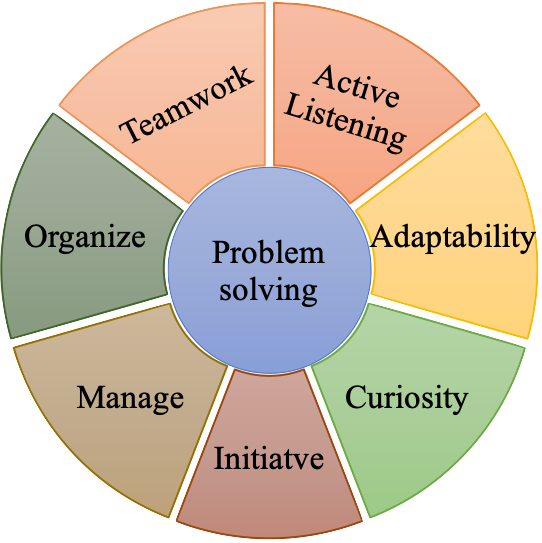
\includegraphics[scale=0.42]{img/personal.png}
~ 
\section{Automation}
~
	NextFlow
	SnakeMake
	Make
~
\end{aside}

\newpage
\section{Fellowship \& Awards}
\begin{entrylist}
\entry
	{2019}
	{Travel grant award}
	{Hjärt-Lungfonden}
	{Heart-Lung Foundation travel grant award to attend 4th International Conference on Innate Immune Memory, Nijemegen, the Netherlands.}
	
\entry
	{2012}
	{Research grant award}
	{Department of Science \& Technology, Govt of India}
	{DST-Inspire fellowhip award by Govt. of India to pursue PhD degree program.}
	
\entry
	{2010}
	{Institute Scholarship}
	{Bose Institute, Kolkata}
	{National Scholarship awarded to pursue PhD program by Bose Institute, Kolkata - an autonomous body undertaken by Govt of India.}
	
\entry
	{2010}
	{University Gold Medal}
	{West Bengal University of Technology}
	{Awarded University Gold Medal for the topper of the batch, M.Tech (BT), 2010.}
	
\entry
	{2008}
	{Graduate Aptitude Test in Engineering}
	{Ministry of Human Resources Development, GOI}
	{\textit{Successfully scored rank where the sucess rate is 12-15\%.}}
\end{entrylist}

\section{Teaching \& Mentoring}
\begin{entrylist}
\entry
	{2019}
	{Organize 3 weeks R workshop for PhD students}
	{Linköping University}
	{Organize the R fundamental workshop for the PhD students (total 18 participants) to understand the data analysis, mangement, statistical analysis and graphical representation of multi-variate data in R in 3 weekly sessions. The workshop is supported by Forum Scientium, LiU}
	
\entry
	{2018}
	{Live imaging of intracellular infections, NDPIA workshop}
	{Linköping University}
	{Mentoring and co-working with a group of students at NDPIA one week's workshop at Department of Clinical and Experimental Medicine.}
	
\entry
	{2019}
	{Expert reviewer}
	{Linköping University}
	{Expert reviewer of one International Master's Program in Medical and Experimental Neurosicence.}
	
\entry
	{2018-19}
	{Mentoring two masters' projects on Bioinformatics}
	{Linköping University}
	{Co-working with Prof. Maria Lerm to guide two master's theses on the bioinformatics part with DNA methylation analysis in R and fundamental of Linux.}
	
\entry
	{2018}
	{Mentoring one master's project on Image analyses}
	{Linköping University}
	{Co-working with Prof Maria Lerm to guide one master's thesis with image analysis and statistical calculations with live imaging techniques.}
	
\entry
	{2015}
	{Course design, teaching and examinar}
	{Bidhannagar Govt College, WB, India}
	{One semester Bioinformatics course curriculum design, deliver lectures and set examination for a group of masters (microbiology) students.}
\end{entrylist}

\begin{aside}
	~
	~
	~
	~
	\section{Professional community }
	\href{https://orcid.org/0000-0002-5649-4658}{
\includegraphics[scale=0.30]{img/orcid}}
	~
	\href{https://scholar.google.com/citations?user=IMBYOv8AAAAJ&hl=en}{
\includegraphics[scale=0.40]{img/gscholar}}
	~
	\href{https://publons.com/researcher/921358/jyotirmoy-das/}{
\includegraphics[scale=0.50]{img/publon}}
	~
	\href{https://www.researchgate.net/profile/Jyotirmoy_Das}{
\includegraphics[scale=0.60]{img/researchgate}}
	~
	\href{https://www.linkedin.com/in/dasjyotirmoy/}{
\includegraphics[scale=0.40]{img/linkedin}}
	~
  \section{Languages}
	\textbf{English}
\includegraphics[scale=0.40]{img/5stars.png}
	\textbf{Hindi}
\includegraphics[scale=0.40]{img/5stars.png}
	\textbf{Bengali}
\includegraphics[scale=0.40]{img/5stars.png}
	\textbf{Swedish}
\includegraphics[scale=0.40]{img/1stars.png}
~	
	\section{Research Interests}
	Functional Genomics
	Genome Assembly
	Sequence Analysis
	Epigenetics
	Big Data Analysis
	Cluster Computing
	Cloud Computing
	Visualization, front-end solution
\end{aside}

\newpage
\section{Poster \& Oral presentation}
\begin{entrylist}
\entry
	{2021}
	{Oral presentation - Clinical Genomics, Sweden}
	{Sigtuna, Stockholm}
	{short oral presentation}
\entry
	{2019}
	{Poster presentation - 4th International Conference on Innate Immune Memory}
	{Radbound University, the Netherlands}
	{poster presented at the international conference.}
\entry
	{2019}
	{Oral presentation - Machine Learning and Epigenetics}
	{Linköping University}
	{Demonstrating the Machine Learning approach towards the big data of epigentics among a group of undergraduate enginnering students (total 16 participants) from Purdue University, USA}
\entry
	{2019}
	{Short oral presentation}
	{MIIC, Linköping University}
	{Short oral presentation to market own research, organized by Mucosal Infection and Inflammation Center. \\ \textit{best presenter award}}
\entry
	{2018}
	{Oral presentation -Advanced Image analysis}
	{Linköping University}
	{Oral presentation in advanced image analysis with MATLAB\textsuperscript{\textregistered}in NDPIA workshop.}
\entry
	{2018}
	{Poster presentation - IKE Day}
	{Linköping University}
	{Poster presentation at the annual IKE day seminar.}
\entry
	{2018}
	{Poster presentation - Tuberculosis research seminar}
	{Karolinska Institute, Stockholm}
	{Poster presentation at the tuberculosis research seminar.}
\end{entrylist}
\begin{aside}
~
~
~
~
	\section{Hobbies}
	
\includegraphics[scale=0.60]{img/hobby}
~	
\end{aside}
\newpage
\section{Referees}
\begin{entrylist}
	\entry
	{\textbf{Referee 1}}
	{Prof. Maria Lerm, \\Professor of Immunology\\Department of Clinical \& Experimental Medicine (BKV)\\Faculty of Health Sciences
		\\Linköping University, Sweden}
	{}
	{Email: \href{mailto: maria.lerm@liu.se}{\textbf{Maria.Lerm}@liu.se}\\
	\emph{Phone: +46 (0)73-270 77 86}}
\\
\entry
	{\textbf{Referee 2}}
	{Prof. Tapas C Ghosh, \\Senior Professor \\ Bioinformatics Center (Center of Excellence), \\Bose Institute, India}
	{}
	{Email: \href{mailto: tapash@jcbose.ac.in}{\textbf{Tapash}@jcbose.ac.in}, \href{mailto: tapashbic@gmail.com}{\textbf{Tapash@gmail.com}}\\
				\emph{Phone: +91 704 477 04 27}}
	\end{entrylist}


%\begin{flushleft}
%\emph{March 31st, 2020}
%\end{flushleft}
%\begin{flushright}
%\emph{Jyotirmoy Das}
%\end{flushright}

\end{document}
